\chapter{Traitement d'images}\label{ficheImage1}  

Un logiciel de traitement d'images permet de retoucher une image existante : taille de l'image, luminosité, contraste, recadrage, etc...\\

\prof{on pourra ici indiquer qu'il existe plusieurs logiciels de traitement d'images, l'un des plus connus étant Photoshop d'Adobe. Le logiciel de traitement d'images utilisé ici est Gimp. Il présente l'avantage d'être libre et gratuit. L'utilisation de nombreuses fonctions est la même pour ces deux logiciels.}

\section*{Synoptique}

{\footnotesize
\begin{itemize}
\item Logiciel\footnote{Le logiciel Gimp est librement téléchargeable : \url{http://www.gimp.org/}} : \emph{Gimp}
\item Prérequis : aucun
\item Matières concernées : arts visuels et histoire-géographie
\item Objectifs : utiliser un logiciel de retouche d'image pour effectuer des modifications sur une image existante puis l'exporter au format JPG ou PNG (documents à rendre sur Teams).
\item Compétences : 
        \begin{itemize}
        \item format d'image JPG et PNG ;
        \item capture d'écran ;
        \item recadrage.
        \end{itemize}
\item Cette fiche est à réaliser :
        \begin{itemize}
        \item avant la fin du semestre de cours en arts visuels ;
        \item après la séance 1 en français  ;
        \item avant la fin du semestre de cours en arts visuels. 
        \end{itemize}
\prof{\item vous devez préparer trois éléments \underline{avant} la séance : \begin{itemize}\item récupérer sur Teams le fichier \texttt{photoFlorimont.png} qui contient une image aérienne de Florimont, sur laquelle les élèves travailleront ;\item mettre à disposition des élèves sur la page Teams de votre cours le fichier \texttt{ExtraitMoliere6e.odt} \item créer un dossier de remise de devoir sur la page Teams de votre classe car les élèves rendent cette activité sous la forme d'un fichier PDF déposé sur Teams.\end{itemize}}
\end{itemize}
}




\newpage

\section{Séance 1 : recadrer une image}\index{Gimp!Recadrer une image}\index{Recadrage d'une image (Gimp)}

\subsection{Premiers pas avec Gimp...}\index{Ouvrir!Gimp}\index{Gimp!Ouvrir}

\prof{par défaut le logiciel Gimp s'ouvre en mode multi-fenêtres, et avec la boîte à outils non activée. Après l'ouverture du logiciel, il faut veiller à ce que tous les élèves aient une interface similaire à celle montrée ci-dessous. Si les différents boîte à outils ne sont pas tout à fait au même endroit, ce n'est pas grave. En effet, l'ordre dans lequel on effectue les opérations détermine la position finale des boîtes d'outils.}

Lancer le logiciel en utilisant la <<\,loupe\,>> :

\uneimageici{./images/generales/loupe}{.7\textwidth}

... puis en indiquant \emph{Gimp} :

\uneimageici{./images/generales/loupeRechercheGimp}{.7\textwidth}


La fenêtre principale du logiciel s'ouvre :

\uneimageici{./images/gimp/GimpInterface}{.7\textwidth}

Si elle ne ressemble pas à celle-ci, alors il faut effectuer les réglages suivants :

\begin{minipage}[c]{.58\textwidth}
\begin{itemize}
\item Ouvrir le menu \texttt{Fenêtre}, puis cocher la case \texttt{Mode fenêtre unique}.
\item Dans le même menu, cliquer également sur \texttt{Boîte à outils} pour faire apparaître les outils.
\end{itemize}
\end{minipage}\hfill%
\begin{minipage}[c]{.38\textwidth}
\uneimageici{./images/gimp/GimpMenuFenetre2}{.9\textwidth}
\end{minipage}




%
%
%  S  É  A  N  C  E     I
%
%






\subsubsection{Pour bien démarrer}

Sur la page Teams de votre cours, récupérer le fichier \texttt{photoFlorimont.png}. Si nécessaire, se reporter à la fiche méthode \emph{Consulter le sujet d'un devoir en pièce jointe}, page \pageref{consulterDevoir}.

Une fois le fichier enregistré sur le \emph{Bureau} de l'ordinateur, revenir dans \emph{Gimp}, cliquer sur le menu \texttt{Fichier}, puis \texttt{Ouvrir}.

\uneimageici{./images/gimp/GimpOuvrirFichier}{.4\textwidth}

Chercher dans la zone \emph{Raccourcis} le \emph{Bureau} : le fichier à ouvrir peut alors être sélectionné dans la zone centrale de la boîte de dialogue :

\uneimageici{./images/gimp/GimpOuvrirFichier2}{.6\textwidth}

Achever l'ouverture en cliquant sur le bouton \texttt{Ouvrir}.

\subsubsection{Pensez à enregistrer régulièrement}

Dès que vous avez ouvert un nouveau document dans \emph{Gimp}, sauvegardez-le au format \texttt{Nom-seance1.jpg} : dans le menu \texttt{Fichier}, choisir \texttt{Enregistrer}. Pendant que vous travaillez, pensez à sauvegarder régulièrement votre travail (raccourci clavier \texttt{Cmd + s}).   

\uneimageici{./images/generales/clavierCmdS}{.4\textwidth}

%\vfill
%\phantom{rien}


\subsection{Sujet de l'activité...}

\vspace{10pt}

\prof{Assurez-vous que tous les élèves ont franchi les premières étapes ci-dessus. Lire ensuite l'énoncé avec les élèves et montrer le résultat attendu (affichage au TBI du résultat). Expliquez bien où trouver le fichier de départ. À partir de ce point, les élèves travaillent chacun à leur rythme.}

\boiteEnonce{Dans cette activité, vous allez recadrer une photographie aérienne de Florimont, dont vous venez de récupérer une version <<\,brute\,>> au format PNG. L'objectif est d'obtenir le résultat suivant :
\begin{center}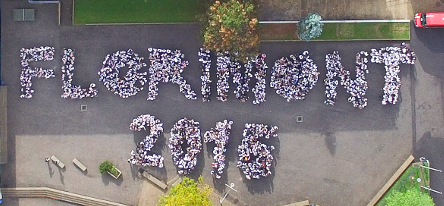
\includegraphics[width=.7\textwidth]{./images/gimp/photoFlorimontReduite}\label{modeleImage}\end{center}
Une fois le cadrage terminé, vous devrez exporter votre fichier au format JPG. Le fichier sera nommé à partir de votre nom : \texttt{Nom-seance1.jpg} et sera rendu sur Teams à l'endroit indiqué par votre enseignant. Si nécessaire, se reporter à la fiche méthode \emph{Remettre son devoir}, page \pageref{TeamsRemettreDevoir}}



\textbf{Pour obtenir de l'aide, rendez-vous à la page \pageref{correction_gimp01}}

\subsection{Pour aller plus loin...}

Si vous avez terminé votre travail, entraînez-vous à réaliser des captures d'écran (voir page \pageref{CaptureEcran}).










\newpage





%
%
%  S  É  A  N  C  E     II
%
%



\section{Séance 2 : recadrer et encadrer une image}\label{ficheImage2}\index{Gimp!Ajouter un cadre autour d'une image}\index{Cadre autour d'une image (Gimp)}

\prof{cette séance a lieu après la séance \no 1 et réutilise les mêmes outils. Vous devez préparer avant la séance une image de votre choix (au format PNG) qui soit en lien avec votre cours du moment (remarque : cette image doit être compatible avec l'ajout d'un cadre de 1\,cm autour (voir la partie qui traite de l'ajout d'un cadre). Cette image doit être mise à disposition des élèves sur la page Teams de votre cours. Demander ensuite aux élèves d'effectuer le recadrage suivant les consignes données ci-dessous. L'image finale, au format JPG, sera récupérée sur Teams (il faut donc préparer un dossier de remise de devoirs).}  

\subsection{Pour bien démarrer...}

Dès que vous avez ouvert un nouveau document dans \emph{Gimp}, sauvegardez-le au format \texttt{Nom-seance2.jpg} : dans le menu \texttt{Fichier}, choisir \texttt{Enregistrer}. Pendant que vous travaillez, pensez à sauvegarder régulièrement votre travail (raccourci clavier \texttt{Cmd + s}).   

\uneimageici{./images/generales/clavierCmdS}{.4\textwidth}

\subsection{Sujet de l'activité...}

\vspace{10pt}

\boiteEnonce{Dans cette activité, vous allez recadrer une image mise à votre disposition par votre professeur sur la page Teams de votre cours, en respectant les consignes qui vous seront données, puis vous aller ajouter un cadre blanc autour de cette image. Cette image, dont vous venez de récupérer une version <<\,brute\,>>, est au format PNG.\newline \\
Une fois l'encadrement terminé, vous devrez exporter votre fichier au format JPG.. Le fichier sera nommé à partir de votre nom : \texttt{Nom-seance2.jpg}) et sera rendu sur la Teams à l'endroit indiqué par votre enseigant. Si nécessaire, se reporter à la fiche méthode \emph{Remettre son devoir}, page \pageref{TeamsRemettreDevoir}}





\subsection{Pour aller plus loin...}

Si vous avez terminé votre travail, entraînez-vous à réaliser des captures d'écran, en sélectionnant une partie de l'écran seulement (voir page \pageref{CaptureEcran}).


\newpage

%
%
%  S  É  A  N  C  E     III
%
%


\section{Séance 3 : recadrer et régler luminosité, contraste}\label{ficheImage3}

\prof{faire réfléchir les élèves sur les différents types de cadrage et l'équilibre d'une composition. Les élèves sont ici libres de choisir leur cadrage ; vous pouvez donc les aiguiller vers un cadrage classique, personnel, ou plus créatif. \underline{Avant la séance}, vous devez déposer l'image brute sur la page Teams de votre cours, et préparer un dossier de remise de devoir. L'image brute pour cette activité est disponible sur Teams.}

\subsection{Pour bien démarrer...}

\vspace{10pt}

Dès que vous avez ouvert un nouveau document dans \emph{Gimp}, sauvegardez-le au format \texttt{Nom-seance3.jpg} : dans le menu \texttt{Fichier}, choisir \texttt{Enregistrer}. Pendant que vous travaillez, pensez à sauvegarder régulièrement votre travail (raccourci clavier \texttt{Cmd + s}).   

\uneimageici{./images/generales/clavierCmdS}{.4\textwidth}

\subsection{Sujet de l'activité...}

\vspace{10pt}

\boiteEnonce{Le but de cet exercice est de retoucher une image représentant un détail des vitraux de la chapelle de l'école dont vous devez récupérer une version <<\,brute\,>> au format PNG sur la page Teams de votre cours. Vous devrez :
\begin{itemize}
\item choisir un cadrage en fonction des consignes données par votre professeur ;
\item régler la luminosité et le contraste selon les indications du paragraphe \vref{GimpLumiContraste} ;
\item ajouter un cadre autour de l'image. 
\end{itemize}\vspace{0.5cm}
}
\vfill
\phantom{rien}
\boiteEnonce{
L'image brute à modifier est la suivante :
\uneimageici{./images/gimp/vitrauxSmall}{.3\textwidth}
Une fois votre travail terminé, vous devrez exporter votre fichier au format JPG (le fichier doit être nommé à partir de votre nom : \texttt{Nom-seance3.jpg}) et le rendre sur Teams, à l'endroit indiqué par votre professeur. Si nécessaire, se reporter à la fiche méthode \emph{Remettre son devoir}, page \pageref{TeamsRemettreDevoir}}









\subsection{Pour aller plus loin}\label{CaptureEcran}\index{Capture d'écran}\index{Gimp!Capture d'écran}

Réaliser une copie d'écran. Il est parfois nécessaire de copier le contenu de l'écran sous forme d'image pour pouvoir l'utiliser dans un document ou une présentation.

\vspace{12pt}

Pour réaliser une copie d'écran :

\begin{enumerate}
\item Capturer l'écran en utilisant un des raccourcis clavier suivant :
        \begin{itemize}
        \item \texttt{Ctrl + Maj + Cmd + 3} pour copier la totalité de l'écran,\index{Raccourci Clavier! Ctrl + Maj + Cmd + 3, copier tout l'écran}
        \item \texttt{Ctrl + Maj + Cmd + 4} pour copier une partie de l'écran (à sélectionner à la souris) ;\index{Raccourci Clavier! Ctrl + Maj + Cmd + 4, copier une partie de l'écran}
        \end{itemize} 

\uneimageici{./images/generales/clavierCapEcran}{.6\textwidth}

\item Coller l'image dans un nouveau document sous \emph{Gimp} : 
\end{enumerate}

\uneimageici{./images/gimp/GimpCollerCommeImage}{.6\textwidth}

On peut alors retravailler l'image comme vous l'avez appris dans cette fiche sur \emph{Gimp}. 





\newpage

\section{Aide pour réaliser les activités}

\subsection{Aide pour la séance 1}


\subsubsection{Utiliser l'outil de découpage}\index{Gimp!Découpage d'une image}\index{Découpage d'une image (Gimp)}\label{correction_gimp01}

Pour découper une partie de l'image afin d'effectuer un recadrage, il faut utiliser l'outil de découpage (icône 
\includegraphics[width=.04\textwidth]{./images/gimp/cutter}) présent dans la boîte à outils.

Sélectionner à l'aide de la souris la zone de l'image à conserver : pour cela, cliquer sur l'image, puis, en maintenant le bouton enfoncé, faire glisser la souris jusqu'à un autre point de l'image. 

\uneimageici{./images/gimp/GimpDecouper1}{.8\textwidth}

La zone sélectionnée est modifiable en déplaçant les 4 angles du rectangle sélectionné. Une fois le cadrage fait, appuyer sur la touche \texttt{Entrée} pour terminer.


\subsubsection{Sauvegarder le fichier}

Il est important de sauvegarder régulièrement le fichier sur lequel on travaille.

Pour enregistrer votre travail :
\begin{itemize}
\item Ouvrir le menu \texttt{Fichier}.
\item Choisir \texttt{Enregistrer sous...}
\item Choisir comme emplacement le \emph{Bureau} de l'ordinateur.
\item Entrer le nom du fichier sous la forme \texttt{Nom-Prénom-date.xcf} \emph{(remarque : XCF est le format de fichier du logiciel Gimp)} 
\item Terminer en cliquant sur \texttt{Enregistrer}.   
\end{itemize}

\uneimageici{./images/gimp/GimpEnregistrerFichier}{.6\textwidth}

Après ce premier enregistrement, pensez à appuyer régulièrement sur la combinaison de touche \texttt{cmd} + \texttt{S} : c'est le \emph{raccourci clavier} permettant d'enregistrer le fichier sur lequel vous êtes en train de travailler.

\uneimageici{./images/generales/clavierCmdS}{.5\textwidth}



\cadre{\textbf{Différence entre \texttt{Enregistrer} et \texttt{Enregistrer sous...}}\newline Dans la plupart des logiciels, on peut : \begin{itemize}\item \textbf{enregistrer} le fichier sur lequel on travaille. Cette opération est possible si le fichier existe déjà et possède un nom. La version courante du fichier sera alors écrite en mémoire et remplacera l'ancienne version du fichier.\item \textbf{enregistrer sous...} le fichier sur lequel on travaille. Cette opération commence par demander un nouveau nom pour l'enregistrement du fichier. On peut donc ouvrir un fichier que l'on ne souhaite pas modifier, choisir \emph{enregistrer sous}, donner un nouveau nom et ainsi travailler sur une copie du fichier de départ.\item utiliser \texttt{cmd + S} (\emph{S} pour \emph{Save}) pour \textbf{enregistrer} le fichier courant. Bien que les documents soient enregistrés automatiquement par la majorité des logiciels, il faut régulièrement sauver son travail pour éviter les surprises.\end{itemize}}






\subsubsection{Exporter l'image dans un autre format}

Il existe de nombreuses manières de coder une image dans un ordinateur. On parle de \emph{format d'image}. Les plus connus et utilisés sont les formats JPG, TIF, PNG et SVG. Ils ont chacun leurs propres caractéristiques, avantages et inconvénients. Dans \emph{Gimp}, les menus \texttt{Enregistrer} et \texttt{Enregistrer sous...} ne permettent que d'enregistrer les images au format XCF. Ce format XCF n'est par contre lisible que par le logiciel \emph{Gimp} ; il faut donc convertir l'image vers un autre format pour qu'elle soit lisible partout. Pour convertir l'image dans un autre format, il faut procéder de la manière suivante : 

\begin{itemize}
\item Ouvrir le menu \texttt{Fichier}.
\item Choisir \texttt{Export As...}
\item Choisir comme emplacement le \emph{Bureau} de l'ordinateur.
\item Comme votre fichier s'appelle déjà \texttt{Nom-Prénom-date.xcf}, \emph{Gimp} propose par défaut comme nom de fichier exporté : \texttt{Nom-Prénom-date.png}. Modifier l'extension du nom de fichier : effacer le \texttt{png} proposé par défaut et le remplacer par \texttt{jpg}.
\item Cliquer sur \texttt{Exporter}.
\item Une deuxième boîte de dialogue s'affiche dans laquelle on peut régler certains paramètres pour la qualité de l'image exportée. On peut garder les valeurs par défaut et cliquer directement sur \texttt{Exporter}.
\end{itemize}
\deuximagesGPici{./images/gimp/GimpExportAs1}{\textwidth}%
		      {./images/gimp/GimpExportAs2}{.8\textwidth}

% SEANCE 2
\subsection{Aide pour la séance 2}


\subsubsection{Ajouter un cadre autour de l'image}\label{GimpCadre}

Pour ajouter un cadre autour de l'image, il faut ajouter de l'espace autour de celle-ci. Cela se fait en modifiant le \emph{canevas} qui est le support de l'image. Quand on agrandit le canevas, on crée un espace vide autour de l'image. Lorsqu'on exportera l'image au format JPG, cet espace sera rempli de blanc.


\begin{minipage}[c]{.38\textwidth}
\begin{itemize}
\item Ouvrir le menu \texttt{Image}.
\item Choisir\\ \texttt{Taille du canevas...}
\end{itemize}
\end{minipage}\hfill%
\begin{minipage}[c]{.58\textwidth}
\uneimageici{./images/gimp/GimpTailleCanevas1}{\textwidth}
\end{minipage}

\begin{minipage}[c]{.38\textwidth}
\begin{itemize}
\item La boîte de dialogue qui s'ouvre indique la taille de l'image en pixels (\texttt{px}).
\end{itemize}
\end{minipage}\hfill%
\begin{minipage}[c]{.58\textwidth}
\uneimageici{./images/gimp/GimpTailleCanevas2}{\textwidth}
\end{minipage}

\begin{itemize}
\item Cliquer sur la case indiquant l'unité (\emph{px}) et choisir \emph{centimètres}.
\item Ajouter 1\,cm à la largeur et à la longueur déjà indiquées.
\item Cliquer sur le bouton \texttt{centrer} pour que l'image soit centrée sur le nouveau canevas plus grand.
\item Cliquer sur \texttt{Redimensionner} pour terminer.
\end{itemize}

\uneimageici{./images/gimp/GimpTailleCanevas3}{.65\textwidth}

La bordure ajoutée autour de l'image est transparente et est représentée par un damier :
\uneimageici{./images/gimp/GimpTailleCanevas4}{.6\textwidth}

Après export au format JPG, on peut constater que la bordure de l'image apparaît bien en blanc.



% SEANCE 3
\subsection{Aide pour la séance 3}


\subsubsection{Luminosité et contraste}\label{GimpLumiContraste}\index{Gimp!Luminosité}\index{Luminosité (Gimp)}\index{Gimp!Contraste}\index{Contraste (Gimp)}


La \textbf{luminosité} d'une image correspond à sa clarté : plus la luminosité est élevée, plus l'image est claire. Plus la luminosité est faible, plus l'image est sombre.

\vspace{12pt}

Le \textbf{contraste} correspond aux différences de luminosité au sein d'une image : plus le contraste est élevé, plus les différences entre les parties lumineuses et les parties sombres de l'image sont marquées.

\vspace{12pt}

Pour régler la luminosité et le contraste d'une image, il faut se rendre dans le menu \texttt{Couleurs} et choisir \texttt{Luminosité-Contraste...} :

\uneimageici{./images/gimp/GimpLuminositeContraste1}{.6\textwidth}

Dans la boîte de dialogue qui s'ouvre, deux curseurs sont disponibles. En bougeant leur position, on peut régler la luminosité ou le contraste de l'image. Les modifications effectuées sont directement visibles à l'écran. Une fois le réglage effectué, cliquer sur le bouton \texttt{Valider} pour terminer.  

\uneimageici{./images/gimp/GimpLuminositeContraste2}{.6\textwidth}



